\newpage
\chapter{\MP method parameters and Simulation Setup}
\label{ch:simSetup}
Now that we know how the \MP method works we will setup a case to get it running. 
We will discuss which options we have in which file and which models are pre-implemented.

\section{\OF \MP method files}
\subsection{\lstinline|kinematicCloudProperties|}
The particles are modeled as a kinematic Cloud. The properties of the particles can be set in \lstinline|kinematicCloudProperties|.
Here we will look at the most important properties.

The first property we can set is the maximal Courant number \lstinline|maxCo| that is used in the Lagrangian time step fraction, see code \ref{code:stepFraction}.
The constant properties, namely the fluid density \lstinline|rho0| and \lstinline|alphaMax| are set. 
The latter is used in \lstinline|createFields| to set the minimum fluid volume fraction that is allowed per cell 
\begin{equation*}
    \fvf_{min} = 1- \fvf_{max}
\end{equation*}
used in equation \eqref{eq:maxAlpha}.
For the particles we set the Drag force model and particle injection in \lstinline|subModels|. 
In \ref{sec:MPLoop} two drag models are discussed: \lstinline|ErgunWenYu| and \lstinline|PlessisMasliyah| which will be tested in the next chapter \ref{sec:paramStudy} as they have an influence on both the fluid and the particulate phase.

Particles can be either placed inside the reactor by \lstinline|manualInjection| or 
For the first we define the particle positions in \lstinline|kinematicCloudPositions|.
For the latter we define a patch through which the particles are injected over a set time.
For both injection types we can set a particle velocity at injection and distribution for the particle diameters.
With \lstinline|nParticle| we set the number of particles in a cell.

In \lstinline|localInteraction| we define how the particles interact with the patches with the elasticity coefficient \lstinline|e| and restitution coefficient \lstinline|mu|.

The packing model defines the particle normal stress mode. In section \ref{sec:MPLoop} we discussed the explicit Harris and Crighton model.
In \OF we can also set the particle normal model to the implicit Harris and Crighton model or the explicit or implicit Lun model.
For the explicit Harris and Crighton model we can set the parameters \lstinline|alphaPacked| as the close packed volume fraction $\pvfcp$, \lstinline|pSolid| as the pressure constant $P_s$, \lstinline|beta| as the exponent and \lstinline|eps| as the small constant limiting how far away from close pack we can get.
We can also add a correction limiting method with the parameter \lstinline|e| which is given by equation \eqref{eq:correctLimiting}.
The collision damping model can be applied by setting \lstinline|dampingModel| to \lstinline|relaxation|. 
In our later simulations it is always set to \lstinline|none| and therefor not applied.

The return-to-isotropy-model is turned on by setting \lstinline|isotropyModel| to \lstinline|stochastic| and turned off by setting it to \lstinline|none|.
We set the close-pack volume for radial distribution function $g_0$ which is used in the relaxation time.
The factor \lstinline|e| determines how elastic the collision is, see $\eta$ in \eqref{eq:DampingTimeG}.

%drag plays big role in coupling



\ifcode
\begin{lstlisting}

/*--------------------------------*- C++ -*----------------------------------*\
| =========                 |                                                 |
| \\      /  F ield         | OpenFOAM: The Open Source CFD Toolbox           |
|  \\    /   O peration     | Version:  plus                                  |
|   \\  /    A nd           | Web:      www.OpenFOAM.com                      |
|    \\/     M anipulation  |                                                 |
\*---------------------------------------------------------------------------*/
FoamFile
{
    version     2.0;
    format      ascii;
    class       dictionary;
    location    "constant";
    object      particleProperties;
}
// * * * * * * * * * * * * * * * * * * * * * * * * * * * * * * * * * * * * * //

solution
{
    active          true;
    coupled         true;
    transient       yes;
    cellValueSourceCorrection off;

    maxCo           1.0;

    interpolationSchemes
    {
        rho.air         cell;
        U.air           cellPoint;
        mu.air          cell;
    }

    averagingMethod dual;

    integrationSchemes
    {
        U               Euler;
    }

    sourceTerms
    {
        schemes
        {
            U           semiImplicit 1;
        }
    }
}

constantProperties
{
    rho0            2526;
    alphaMax        0.9;
}

subModels
{
    particleForces
    {
        PlessisMasliyahDrag
        {
            alphac alpha.air;
        }
        gravity;
    }

    injectionModels
    {
        model1
        {
            type            manualInjection;
            massTotal       0;
            parcelBasisType fixed;
            nParticle       1;
            SOI             0;
            positionsFile   "kinematicCloudPositions";
            U0              (0 0 0);
            sizeDistribution
            {
                type        fixedValue;
                fixedValueDistribution
                {
                    value   0.0025;
                }
            }
        }
    }

    dispersionModel none;

    patchInteractionModel localInteraction;

    localInteractionCoeffs
    {
        patches
        (
            top
            {
                type rebound;
                e    0.97;
                mu   0.09;
            }
            bottom
            {
                type rebound;
                e    0.97;
                mu   0.09;
            }
            walls
            {
                type rebound;
                e    0.97;
                mu   0.09;
            }
            frontAndBack
            {
                type rebound;
                e    0.97;
                mu   0.09;
            }
        );
    }

    heatTransferModel none;

    surfaceFilmModel none;

    packingModel explicit;

    explicitCoeffs
    {
        particleStressModel
        {
            type HarrisCrighton;
            alphaPacked 0.65;
            pSolid 10.0;
            beta 2.0;
            eps 1.0e-7;
        }
        correctionLimitingMethod
        {
            type absolute;
            e 0.9;
        }
    }

    implicitCoeffs
    {
        alphaMin 0.0001;
        rhoMin 1.0;
        applyLimiting true;
        applyGravity false;
        particleStressModel
        {
            type HarrisCrighton;
            alphaPacked 0.65;
            pSolid 5.0;
            beta 2.0;
            eps 1.0e-2;
        }
    }

    dampingModel none; //relaxation;

    relaxationCoeffs
    {
        timeScaleModel
        {
            type nonEquilibrium;
            alphaPacked 0.65;
            e 0.9;
        }
    }

    isotropyModel stochastic;

    stochasticCoeffs
    {
        timeScaleModel
        {
            type isotropic;
            alphaPacked 0.65;
            e 0.9;
        }
    }

    stochasticCollisionModel none;

    radiation off;
}


cloudFunctions
{}


// ************************************************************************* //
\end{lstlisting}
\fi


\subsection{Geometry}
\subsection{Boundary constions}
Inlet is an interstialVelocityInlet which scales the inlet velocity with the volume fraction of air:
\begin{equation*}
    \u_{inlet} = \dfrac{\u}{\fvf}
\end{equation*}

\section{Experimental fluidized bed reactor}
We model the

\begin{figure}[h!]
  \centering
  \hspace{2cm}
  \begin{tikzpicture}
    \node[anchor=center] (img) at (0,2) {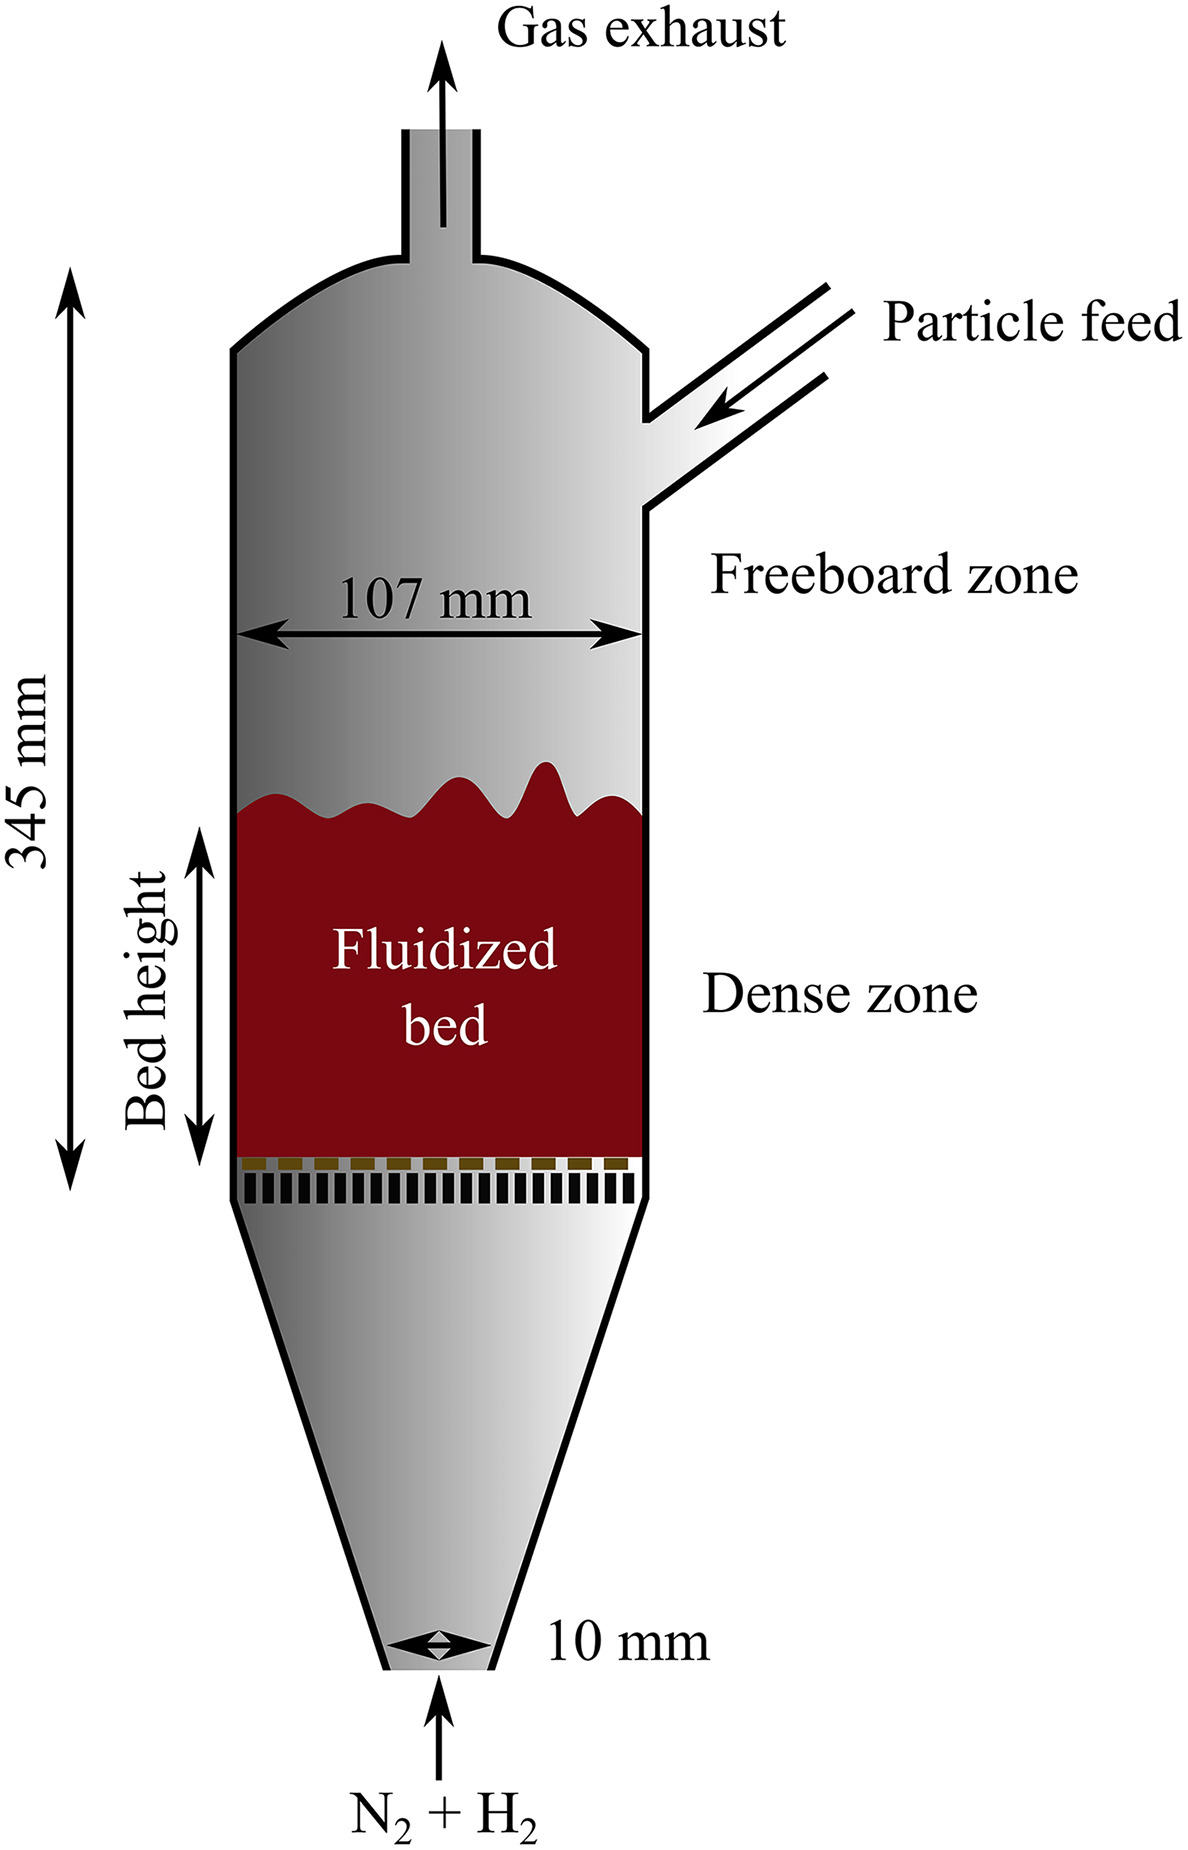
\includegraphics[width=0.4\linewidth]{sections/Setup/1-s2.0-S0016236125021477-gr3_lrg.jpg}};
    % Arrow to bottom-left of the image
    \node[anchor = center] (img2) at (10,2) {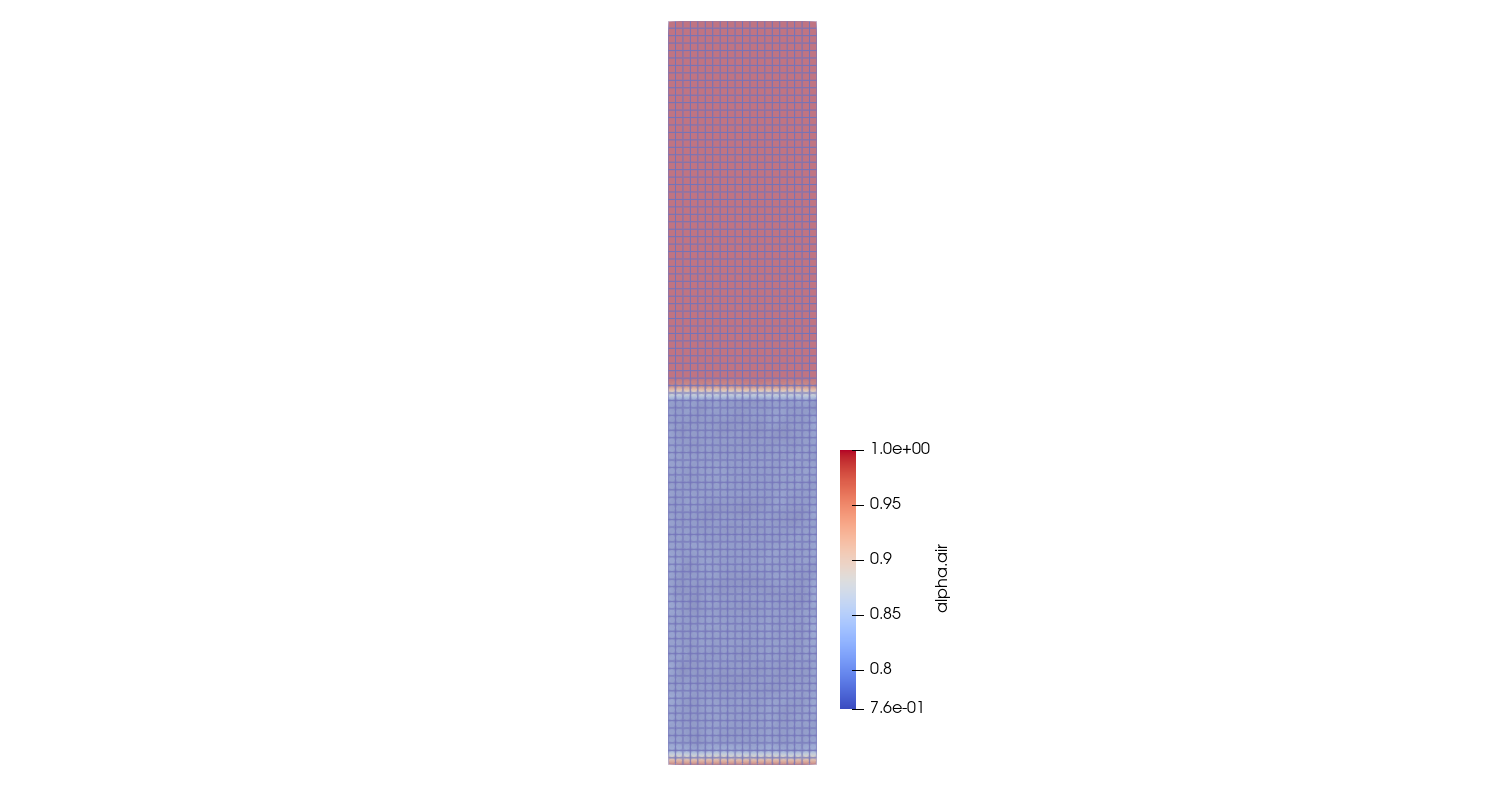
\includegraphics[width=\linewidth]{sections/Setup/geometry_1cm.png}};
    \draw[line width = 3pt, red, dotted] ($(img.south west)+(1.375cm,3.9cm)$) -- ($(img.north west)+(1.375cm,-1.975cm)$) -- ($(img.north east) + (-3.05cm, -1.975cm)$) -- ($(img.south east)+ (-3.05cm, 3.9cm)$) --cycle;
    \draw[->, line width=6pt, red] ($(img2.west)-(-1.5cm,-0cm)$) --($(img.east)+(4cm,0cm)$) ;
    \node (cap) at ($(img.south east)+(-2cm,+0.5cm)$) {\small From: \cite{malte}};
  \end{tikzpicture}
\end{figure}




\subsection{Simplified fluidized bed reactor for comparison}


% \begin{figure}
%     \centering
%     \begin{subfigure}{0.4\textwidth}
%          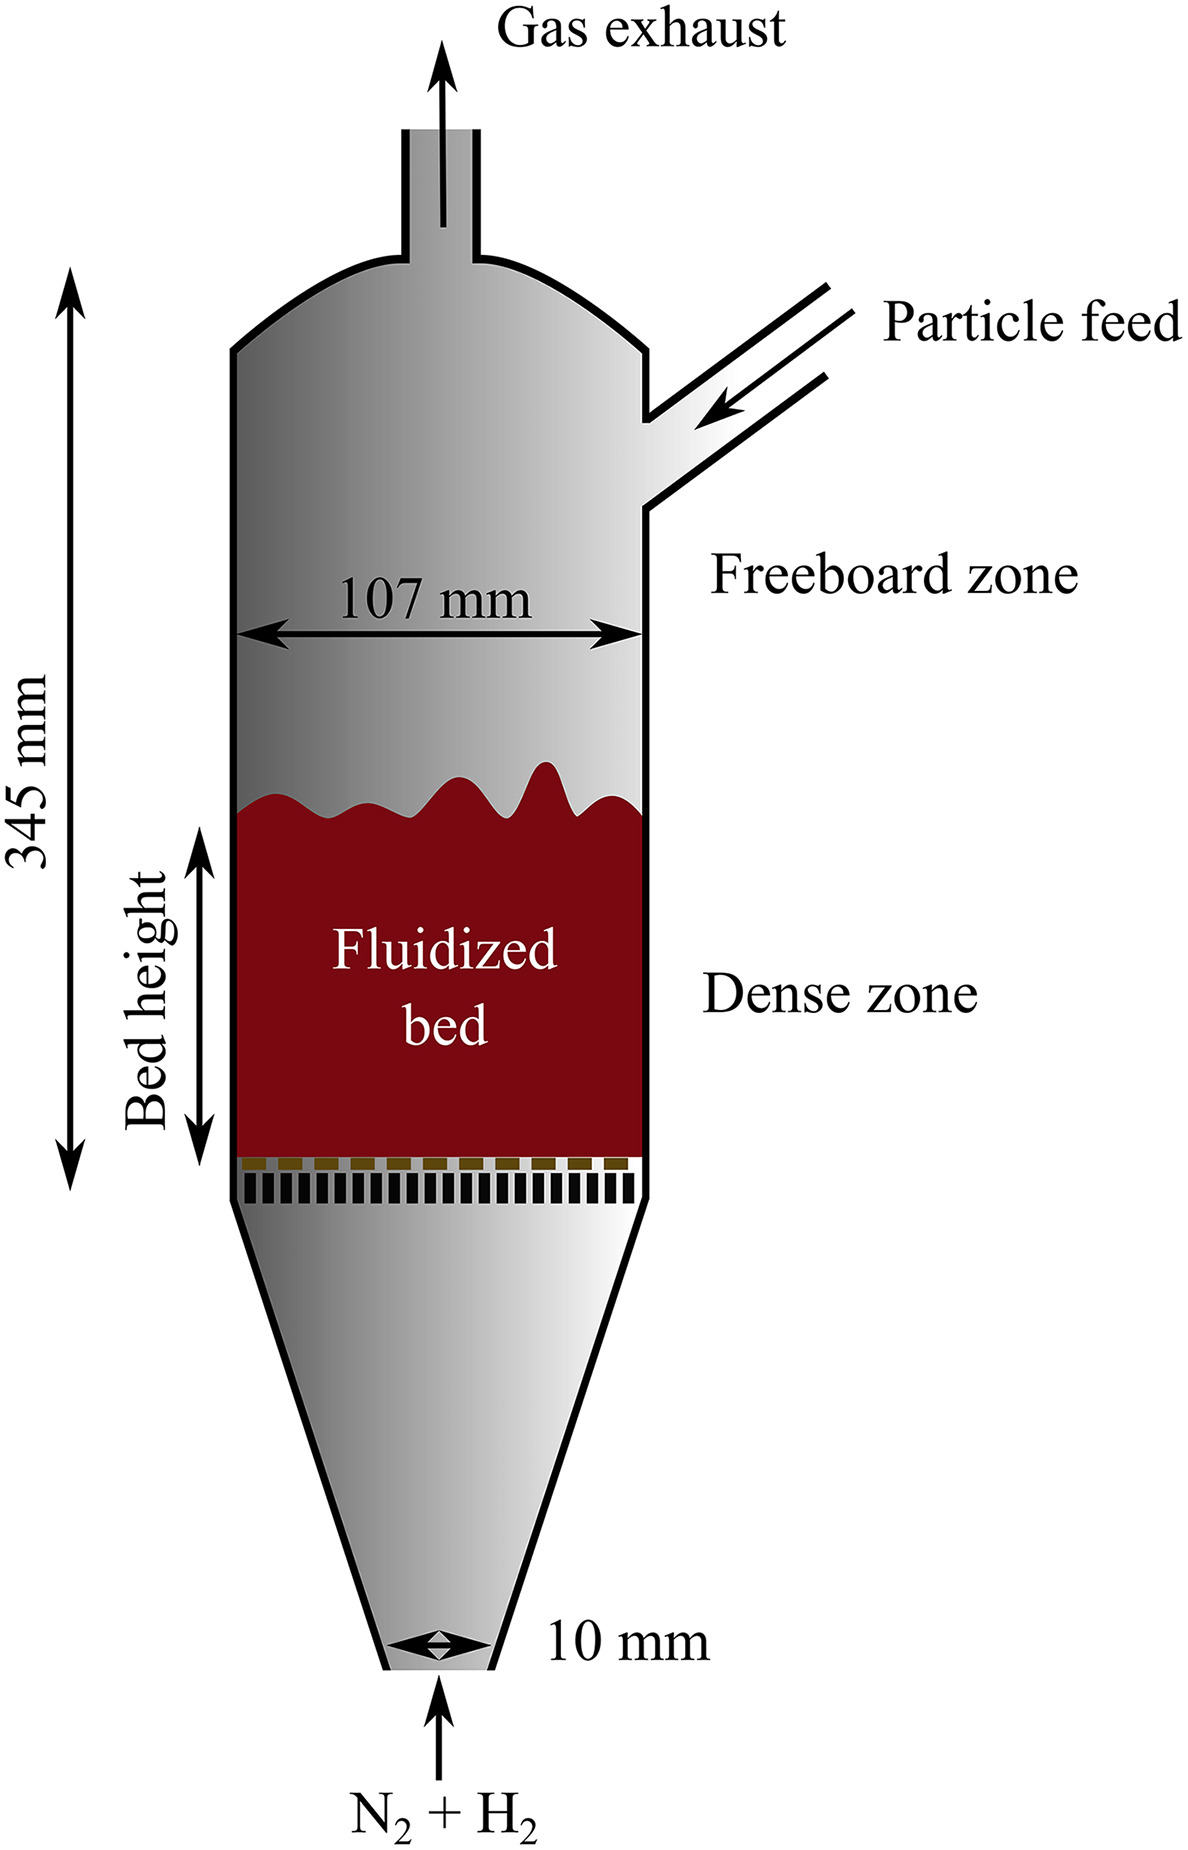
\includegraphics[width=0.8\linewidth]{sections/Setup/1-s2.0-S0016236125021477-gr3_lrg.jpg}
%     \end{subfigure}
%     \begin{subfigure}{0.55\textwidth}
%         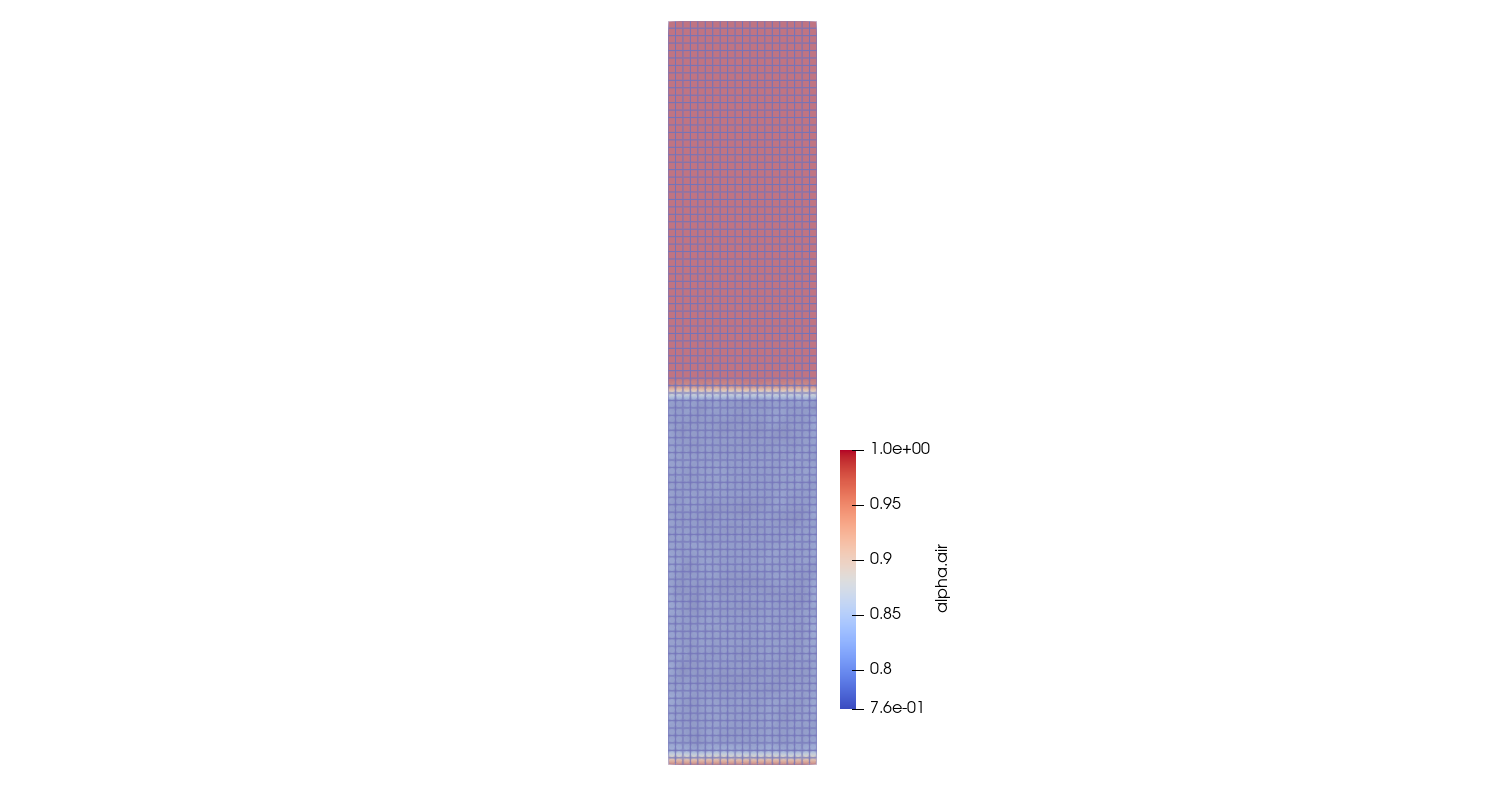
\includegraphics[width=1.5\linewidth]{sections/Setup/geometry_1cm.png}
%     \end{subfigure}
%     \caption{Caption}
%     \label{fig:placeholder}
%\end{figure}



\begin{figure}[h!]
    \centering
    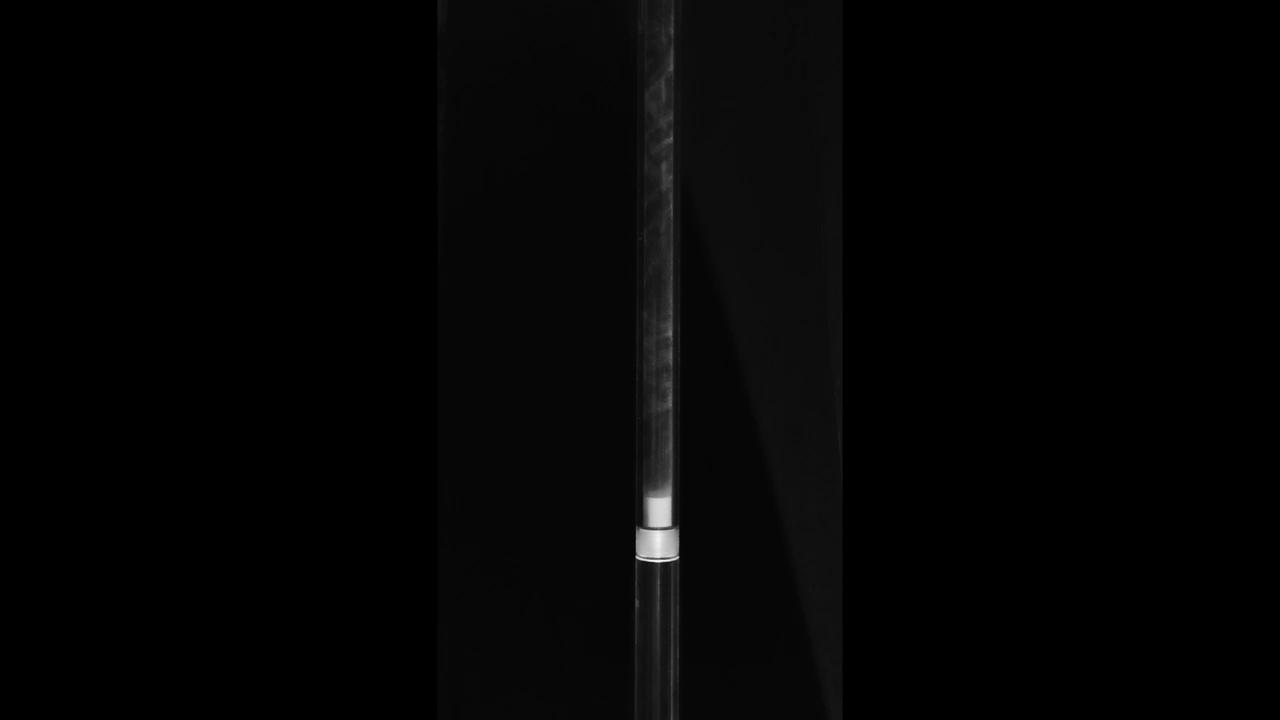
\includegraphics[width = 0.45\linewidth,trim = {15cm 3cm 14cm 4cm},clip]{sections/Setup/003_grey02.png}
    \hfill
    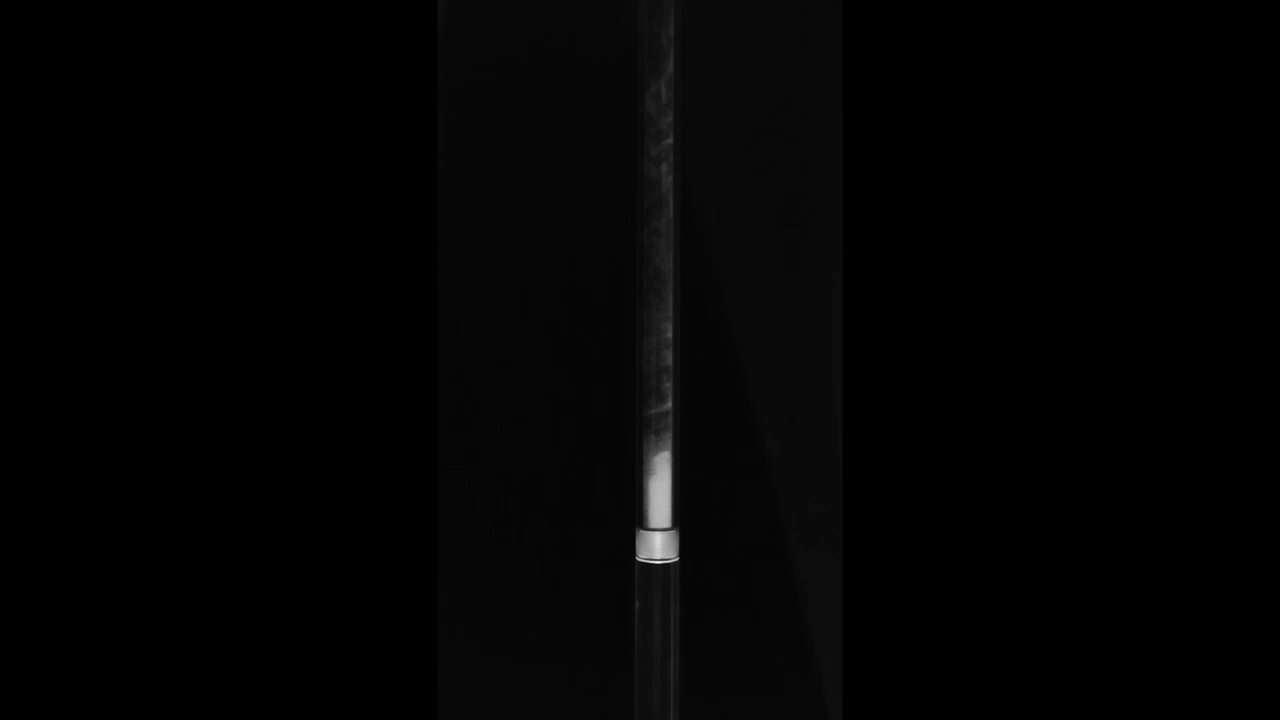
\includegraphics[width=0.45\linewidth,trim = {15cm 3cm 14cm 4cm},clip]{sections/Setup/03_grey48.png}
    \caption{Fluidized bed with glass beads at $u = 0.006m/s$ and $0.06m/s$ inlet velocity}
    \label{fig:placeholder}
\end{figure}


% \begin{figure}
%     \centering
% \begin{tikzpicture}
%     \node[anchor=center] (img) at (0,2) {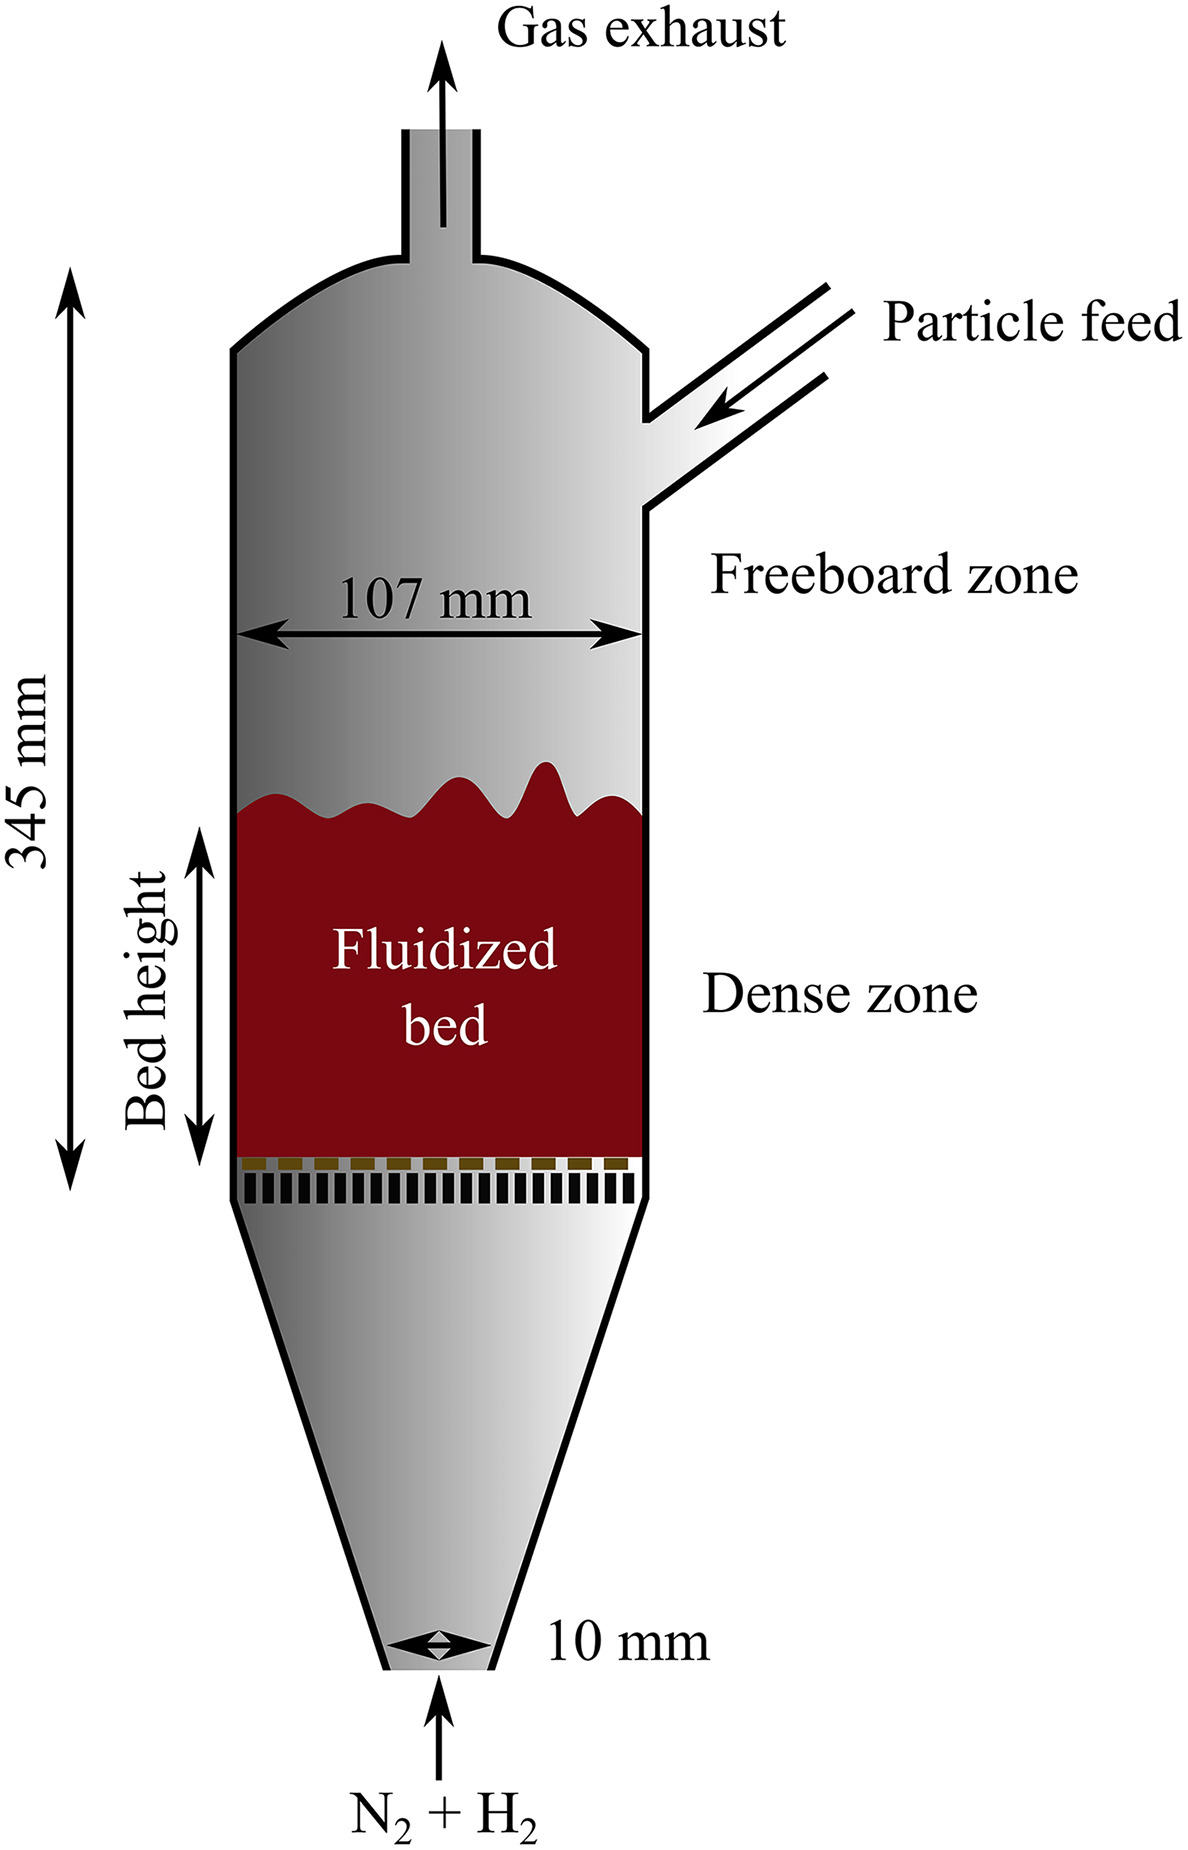
\includegraphics[width=0.25\textwidth]{sections/Setup/1-s2.0-S0016236125021477-gr3_lrg.jpg}};
%     % Arrow to bottom-left of the image
%     \node[anchor = center] (img2) at (8,2) {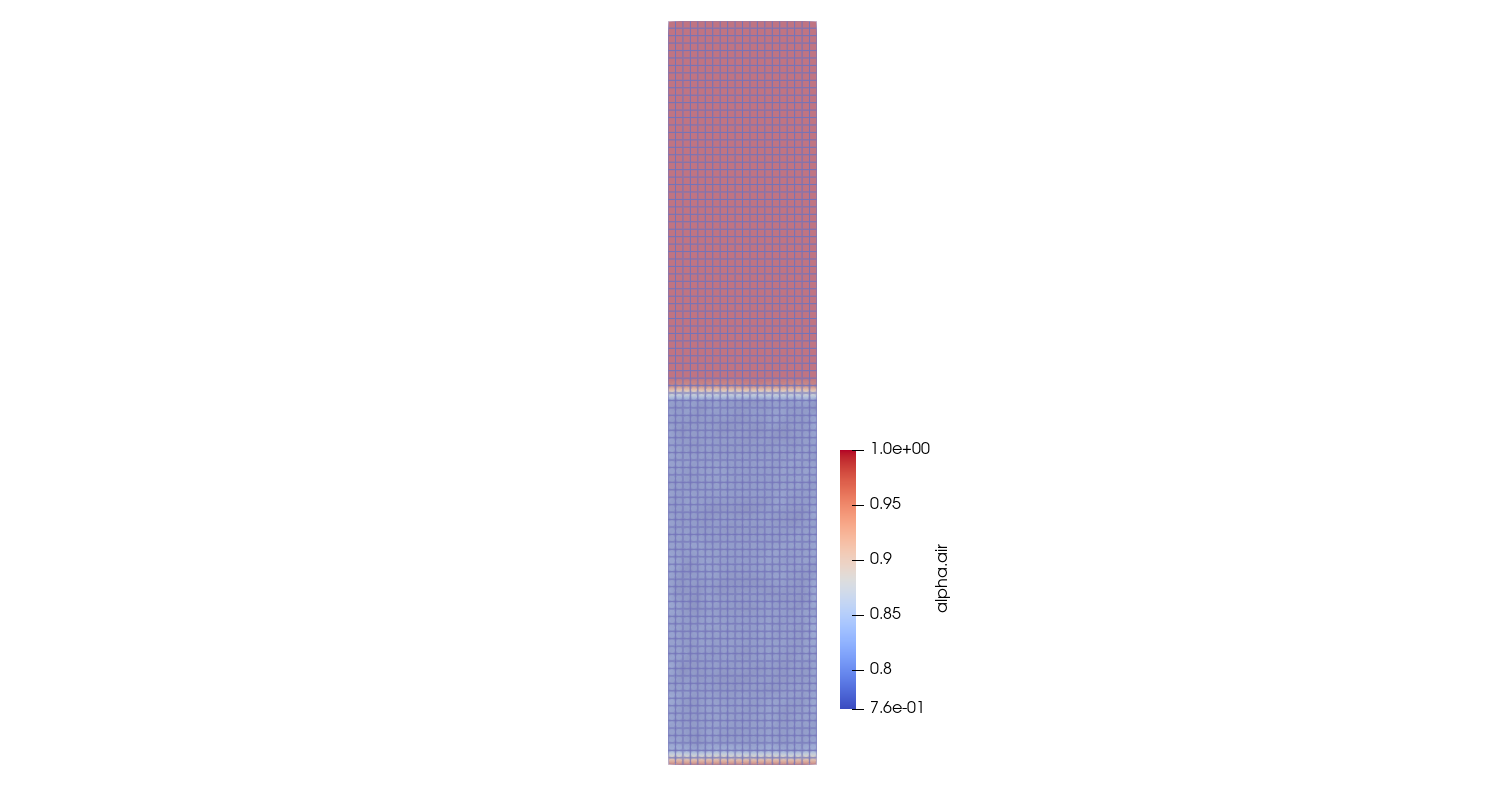
\includegraphics[width = 0.45\textwidth,trim={10cm 0 10cm 0} ,clip]{sections/Setup/geometry_1cm.png}};
%     %\draw[line width = 5pt, red] ($(img.south west)+(4.1cm,2.8cm)$) -- ($(img.north west)+(2.1cm,-3cm)$) -- ($(img.north east) + (-4.6cm, -3cm)$) -- ($(img.south east)+ (-4.6cm, 5.8cm)$) --cycle;
%     \draw[->, line width=10pt, red] ($(img2.west)$) --($(img.east)$) ;
%     \node (cap) at ($(img.south east)+(-2cm,+0.5cm)$) {\small From: \cite{malte}};
%   \end{tikzpicture}
% \end{figure}

\subsection{Mesh}
The highest mean bed height from the data is about $2.4 \operatorname{cm}$. 
To include inflections from the particle we roughly double the height for the simulation using $5 \operatorname{cm}$ as the height of our mesh.
The width of our simulation mesh is adapted to the simplified fluidized bed with $1 \operatorname{cm}$.
Looking at the following mesh study, where we tested grid sizes of two times particle diameter up to twenty times.
\begin{table}[h!]
    \centering
    \begin{tabular}{c|c}
       $\Delta \x /d_p$  & $\Delta \x$ \\
       \hline
        $20$ & $1 \operatorname{mm}$ \\
        $10$ & $0.5 \operatorname{mm}$ \\
        $5$ & $0.25 \operatorname{mm}$ \\
        $4$ & $0.2 \operatorname{mm}$ \\
        $2$ & $0.1 \operatorname{mm}$
    \end{tabular}
    \caption{Caption}
    \label{tab:placeholder}
\end{table}
For a velocity of $0.001 m/s$ we expect to see no fluidization. We expect the particles to drop and lay in a bed.
In the figure \Todo{Referenz}
we can see that for a grid size of $1 \operatorname{mm}$ the particles are flung through the reactor multiple times.
The behavior is less prevalent for a grid size of $0.5 \operatorname{mm}$ but still occurs at later time steps.
For the next two options the difference is nearly indistinguishable. To mitigate simulation costs we therefor choose a cell length of $0.25 \operatorname{mm}$ for all cells.
The simulation is one cell deep leading to a mesh of size $10 \operatorname{mm} \times 0.25 \operatorname{mm} \times 50 \operatorname{mm}$, see 
\Todo{Noch ein Bild}



\section{\lstinline|Goldschmidt| case}

